\documentclass[11pt]{article}
\addtolength{\oddsidemargin}{-1.cm}
\addtolength{\textwidth}{2cm}
\addtolength{\topmargin}{-2cm}
\addtolength{\textheight}{3.5cm}

\usepackage[pdftex]{graphicx}
\usepackage{hyperref}
\usepackage{cleveref}
\usepackage{float}
\usepackage{cite}
\usepackage{placeins}
\usepackage{booktabs}
\hypersetup{
	colorlinks=true,
	linkcolor=black,
	filecolor=magenta,
	urlcolor=cyan,
}

% define the title
\author{Team CodeX}
\title{User Manual}

\begin{document}
	\setcounter{tocdepth}{6}
	\setcounter{secnumdepth}{6}
	\setlength{\parskip}{6pt}
	
	% generates the title
	\begin{titlepage}
	
	\begin{center}
		% Upper part of the page       
		
\includegraphics[width=0.7\linewidth]{../Images/eVoting_Logo.png}\\[2cm]    
		\textsc{\LARGE Electronic Voting}\\[0.5cm]
		% Title
		\rule{\linewidth}{0.5mm} \\[1cm]
		{ \huge \bfseries User Manual}\\[0.5cm]
		\rule{\linewidth}{0.5mm} \\[1cm]
		
		% Author and supervisor
<<<<<<< HEAD
		
\includegraphics[width=0.5\linewidth]{../Images/TeamCodexLogo.jpg}\\[0.5cm]    	
=======
		
		
\includegraphics[width=0.5\textwidth]{../Images/TeamCodexLogo.jpg}\\[0.5cm]    	
>>>>>>> 9b25dd959830e00c0e449a84c7623c3e326c347b
		
		
		\begin{minipage}{0.4\textwidth}
			\begin{flushleft} \large
				Andreas {du Preez}
			\end{flushleft}
		\end{minipage}
		\begin{minipage}{0.4\textwidth}
			\begin{flushright} \large
				\emph{} \\
				12207871 
			\end{flushright}
		\end{minipage}
		
		
		\begin{minipage}{0.4\textwidth}
			\begin{flushleft} \large
				\emph{} \\
				Azhar {Mohungoo }
			\end{flushleft}
		\end{minipage}
		\begin{minipage}{0.4\textwidth}
			\begin{flushright} \large
				\emph{} \\
				12239799
			\end{flushright}
		\end{minipage}
		
		
		\begin{minipage}{0.4\textwidth}
			\begin{flushleft} \large
				\emph{} \\
				Gift {Sefako }
			\end{flushleft}
		\end{minipage}
		\begin{minipage}{0.4\textwidth}
			\begin{flushright} \large
				\emph{} \\
				12231097
			\end{flushright}
		\end{minipage}
		
		\textsc{\Large Stakeholders}\\[1cm]	
				
		\begin{minipage}{0.4\textwidth}
			\begin{flushleft} \large
				\emph{} \\
				Epi-Use Advance
			\end{flushleft}
		\end{minipage}
		\begin{minipage}{0.4\textwidth}
			\begin{flushright} \large
				\emph{} \\
				Roelof Nuade
			\end{flushright}
		\end{minipage}
		
	\end{center}
\end{titlepage}
	
	\renewcommand{\thesection}{\arabic{section}}
	\newpage
	
	\tableofcontents
	
	\textsc{}\\[1cm]
	
	\newpage
	\section{General Information}
	\subsection{System Overview}
	Electronic Voting, or eVoting for short, is a system which does exactly what the name suggest. It allows members of a demographic country to vote for a political party during an election period. It does so that each vote is completely anonymous by using Blockchain technology.\newline\newline
	The system is usable via an online web page and an Android(4.4+) application.\newline\newline
	There are essentially 4 types of users: An Administrator, a Political Party, an Activator and a Voter. Each having their own dedicated functionality. An administrator user can add a political party user, add an activator user, and deactivate a voter account. A political party account can only check the number of votes they currently have. An activator can only activate a user. And a voter can cast votes.\newline\newline
	In order to make Electronic Voting safe and trustworthy, the activator user is needed. Initially when a new user is registered, they will automatically be 'deactivated', which prevents them from casting any type of vote. This is to prevent a voter from creating a bunch of fake accounts and using those fake accounts to vote multiple times. An activator first need to verify the identity of a voter by providing proof of identity (a drivers license or ID document), after which a voter is then activated and will be granted 2 votes: one vote for a national party, and one vote for a provintial party.\newline\newline
	If a user has not registered yet, they can do so on the web site or on the Android application. Apon registration, the user need to provide: a valid ID number, a password used to log into the system, a name, a surname, the location their registered in (pre defined list of values eg. Pretoria, Johannesburg etc), a mobile number and an email address. A voter is the only user type that can register itself, an activator, political party and administrator can only be added by an existing administrator.\newline\newline
	The beautifull part of eVoting is that it uses Blockchain technology, the same technology used in the famous Bitcoin currency. A blockchain is a distributed database that maintains a continuously-growing list of records called blocks secured from tampering and revision. A more indepth description is beyond the scope of this document.
	
	\subsection{System Configuration}

	\subsection{Installation}
	The Android application can be installed by running the APK file located on our Github at the location:  ClientSide/Android APK/eVoting.apk. An Android version of 4.4 or higher is required.\newline
					\begin{figure}[H]
						\centering
						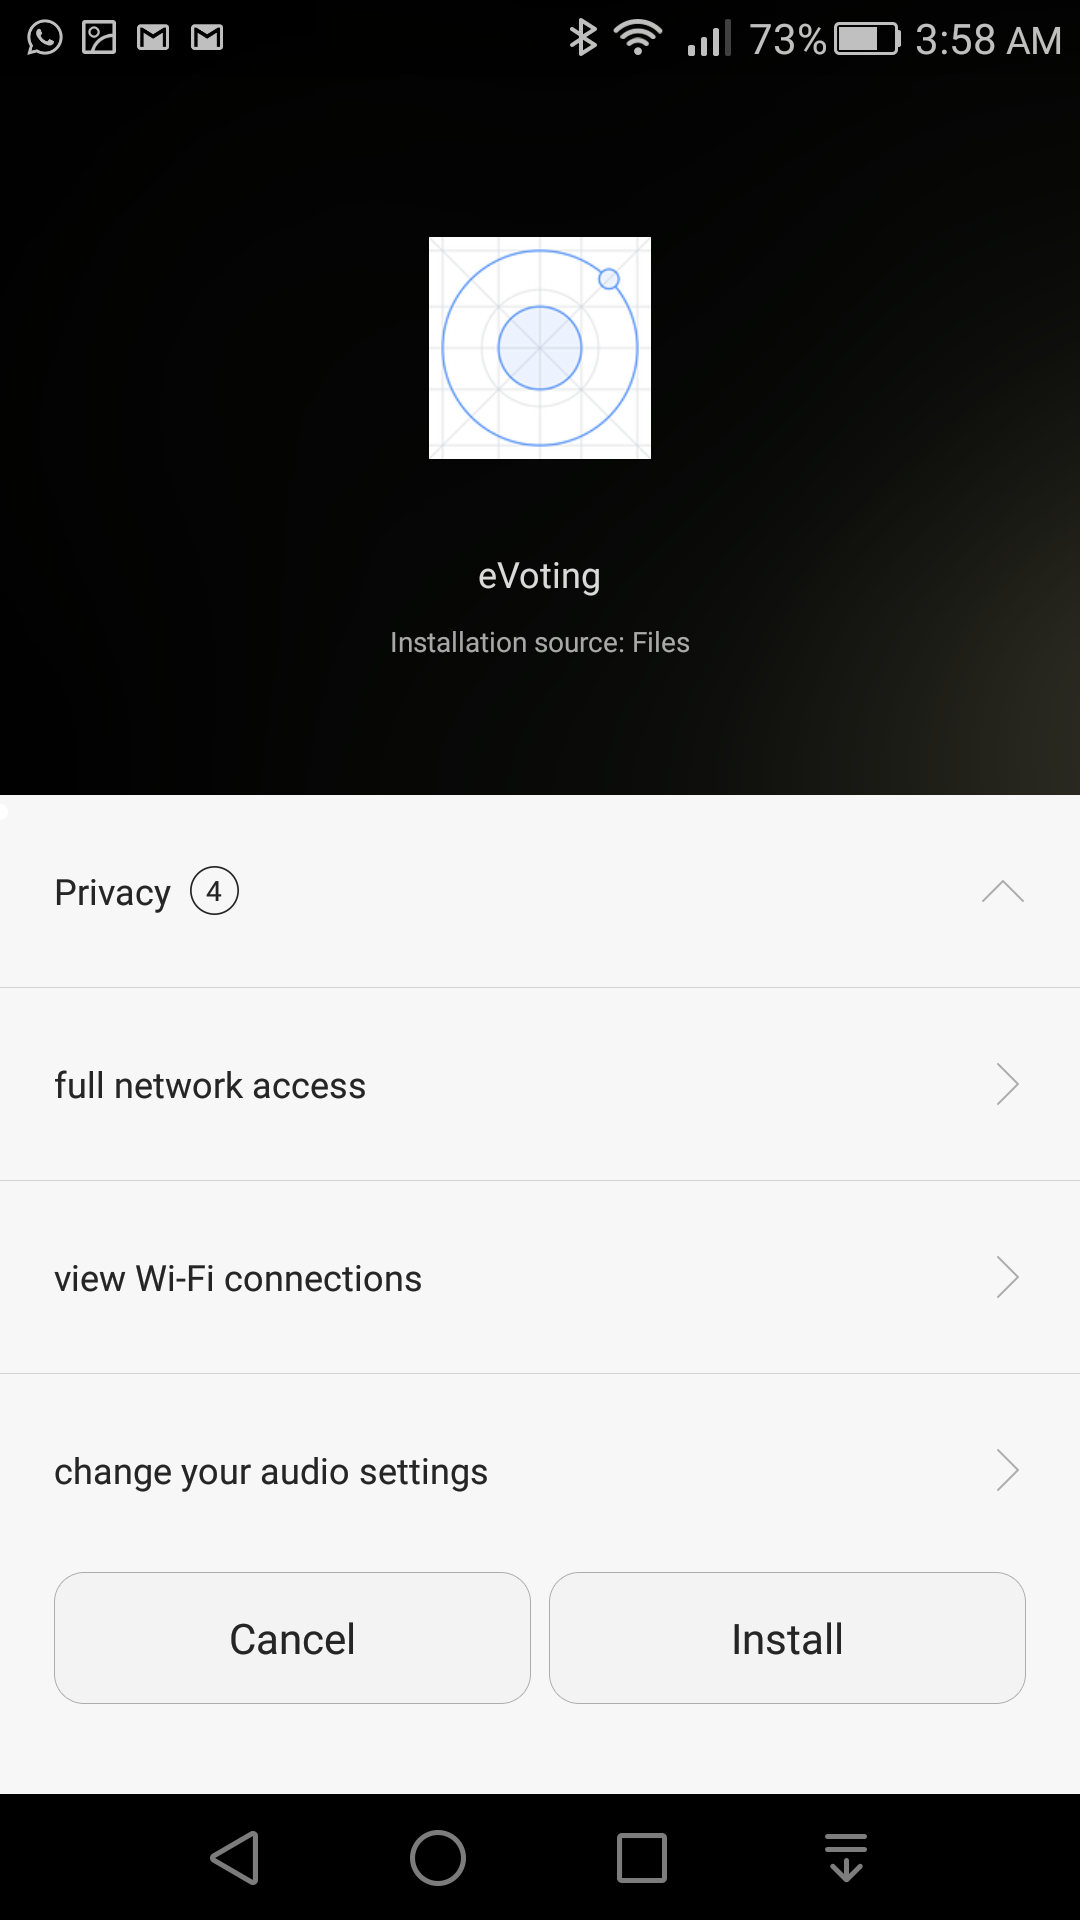
\includegraphics[width=0.3\linewidth]{../Images/UserManual/install.png}
						\caption{Install}
					\end{figure}
					
	The website does not need installation and need only the be viewed inside a web browser which supports HTML5 and Javascript.
	
	\section{Getting Started}
	Getting started with the Android app:\newline\newline
							\begin{figure}[H]
								\centering
								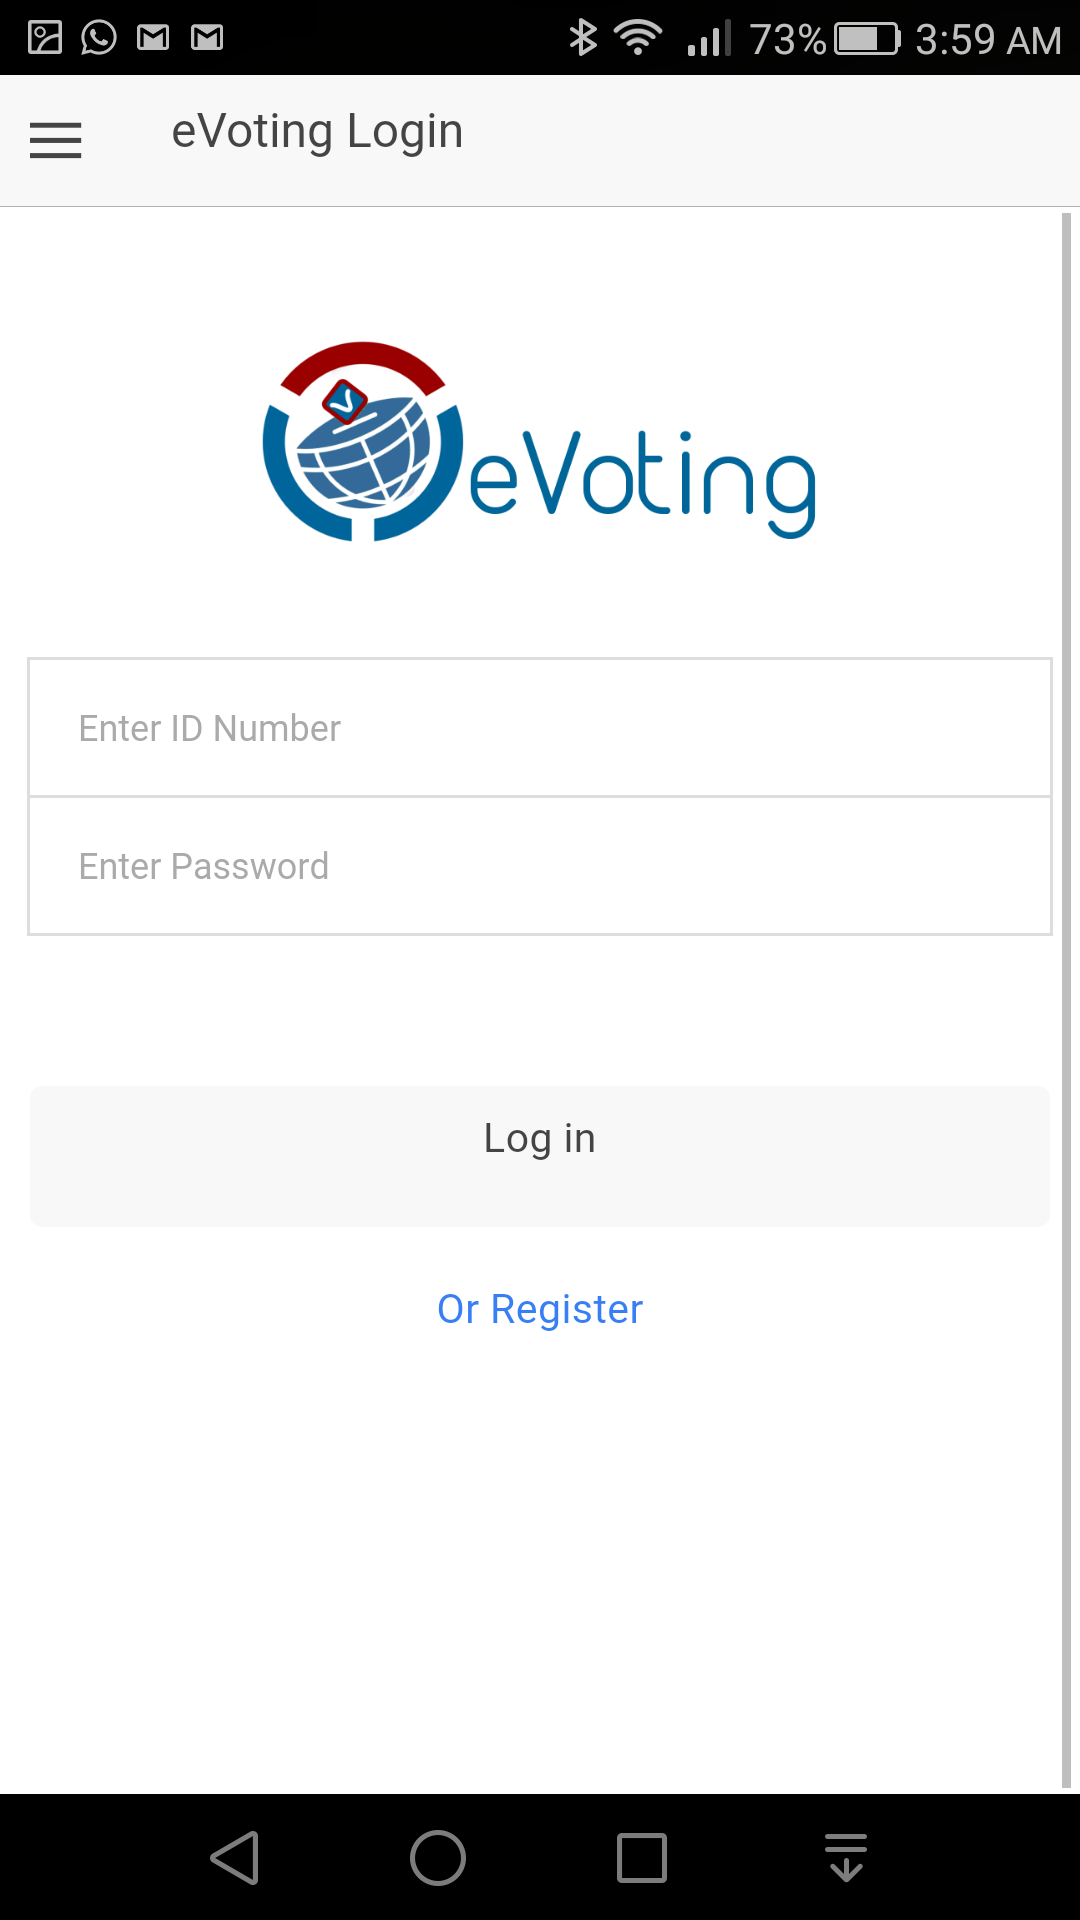
\includegraphics[width=0.3\linewidth]{../Images/UserManual/landingpage.png}
								\caption{Landing Page}
							\end{figure}
	First the user needs to register by clicking on the "Or Register" button at the landing screen.\newline
								\begin{figure}[H]
									\centering
									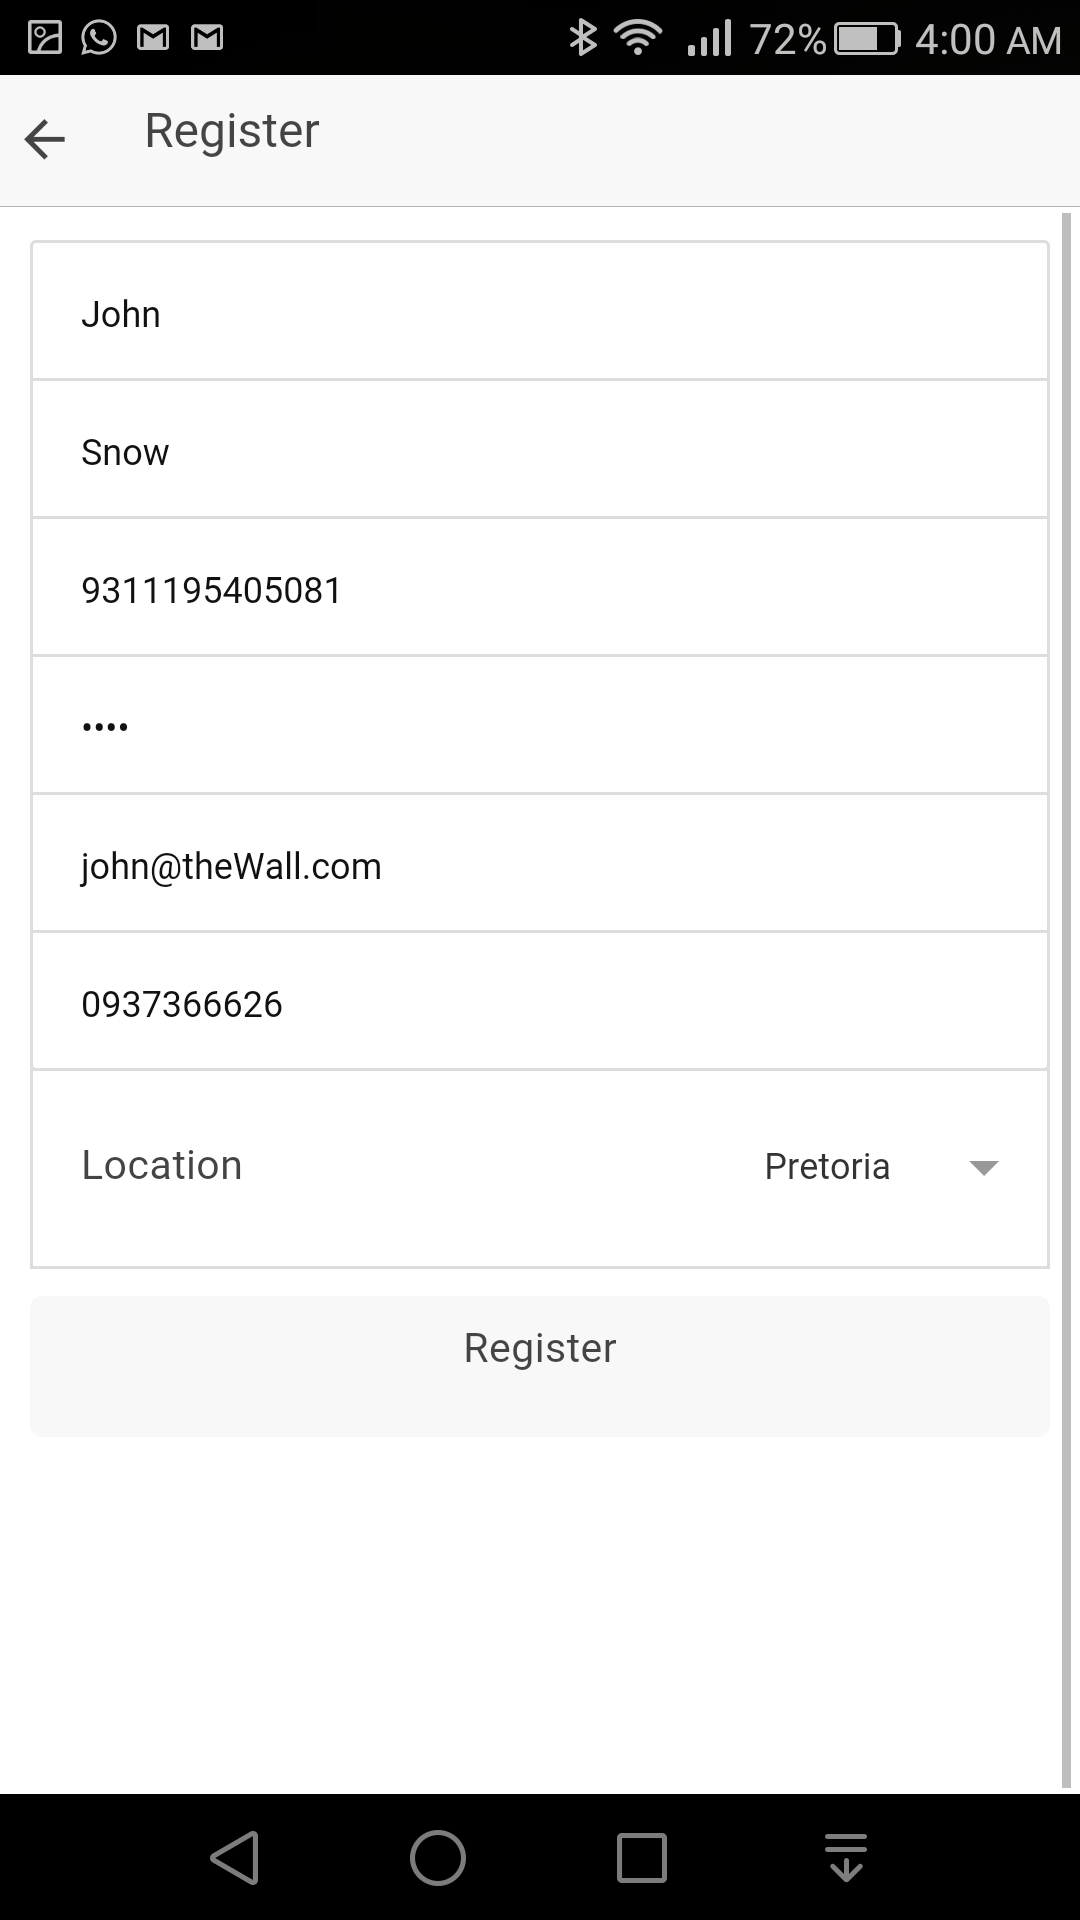
\includegraphics[width=0.3\linewidth]{../Images/UserManual/register.png}
									\caption{Register}
								\end{figure}
	 The user then needs to fill all of the fields then click "Register". Note that no duplicate ID number, email address or mobile number is allowed. If the app gives a popup message stating that the registration is successful, he/she must go back to the landing screen, and log in with their credentials.								\begin{figure}[H]
	 	\centering
	 	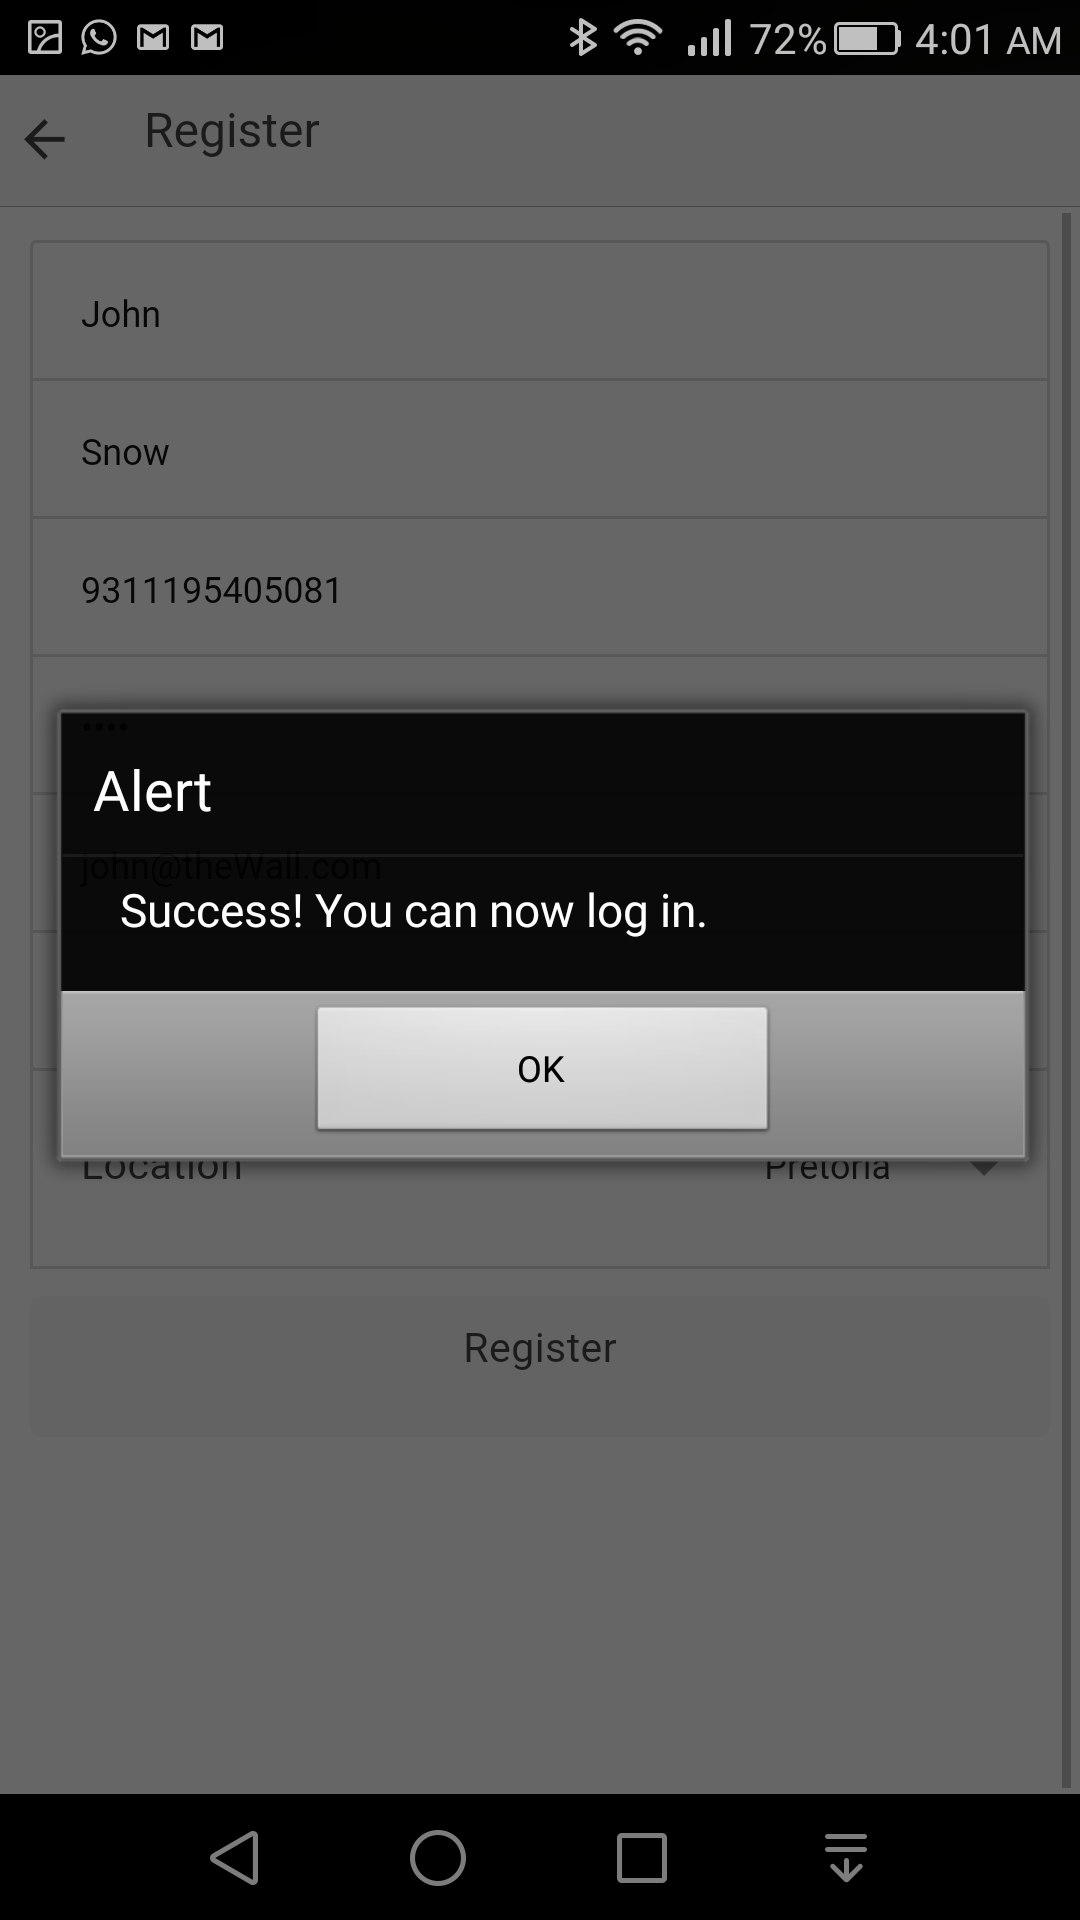
\includegraphics[width=0.3\linewidth]{../Images/UserManual/registered.png}
	 	\caption{Registered}
	 \end{figure}
	The user will then be taken to the home screen. More detail about the home screen can be found in section \ref{homescreen}.\newline
	The app has a side menu which can be accessed by swiping right while logged into the system.\newline
	
	\begin{figure}[H]
		\centering
		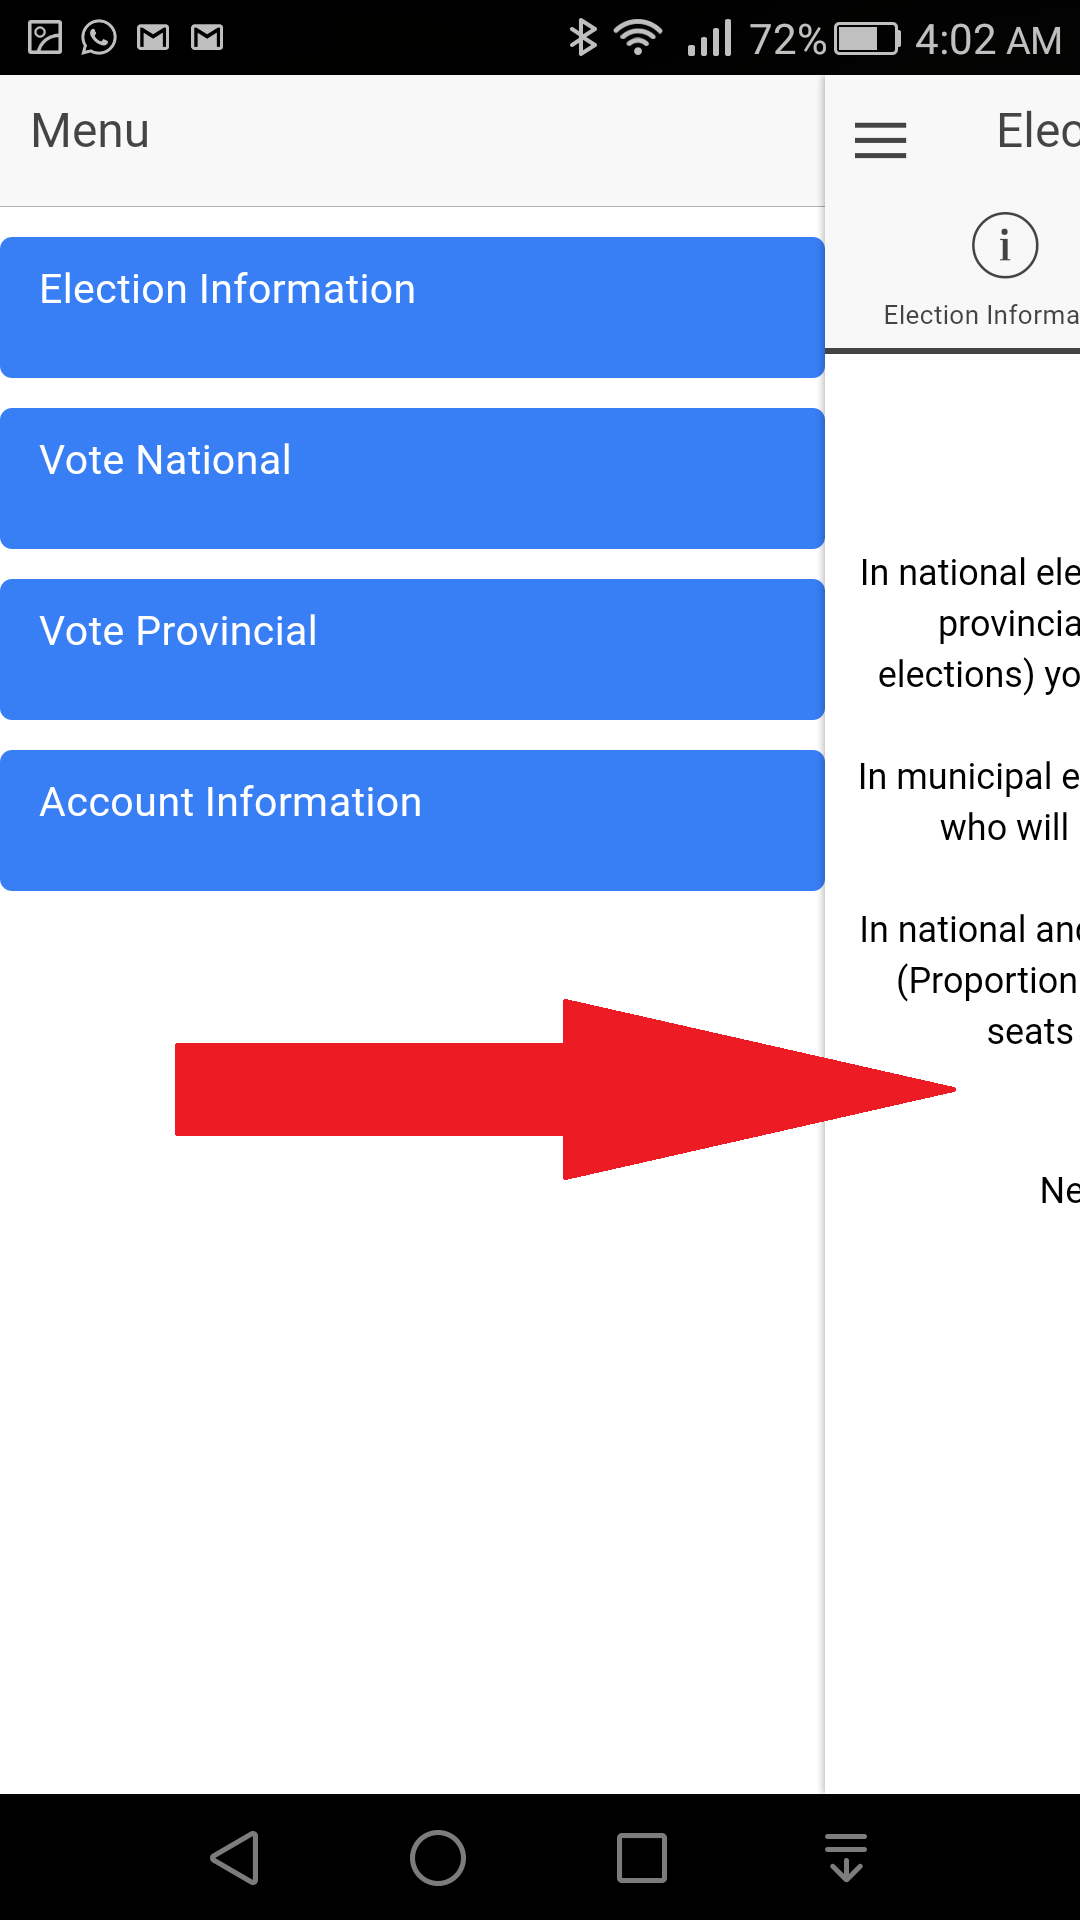
\includegraphics[width=0.3\linewidth]{../Images/UserManual/sidemenu.png}
		\caption{Side Menu}
	\end{figure}
	
	To log out of the system, and tap on "Account Information" in the side menu. Here all of the user's details can be found, as well as a "Log out" button.
	
		\begin{figure}[H]
			\centering
			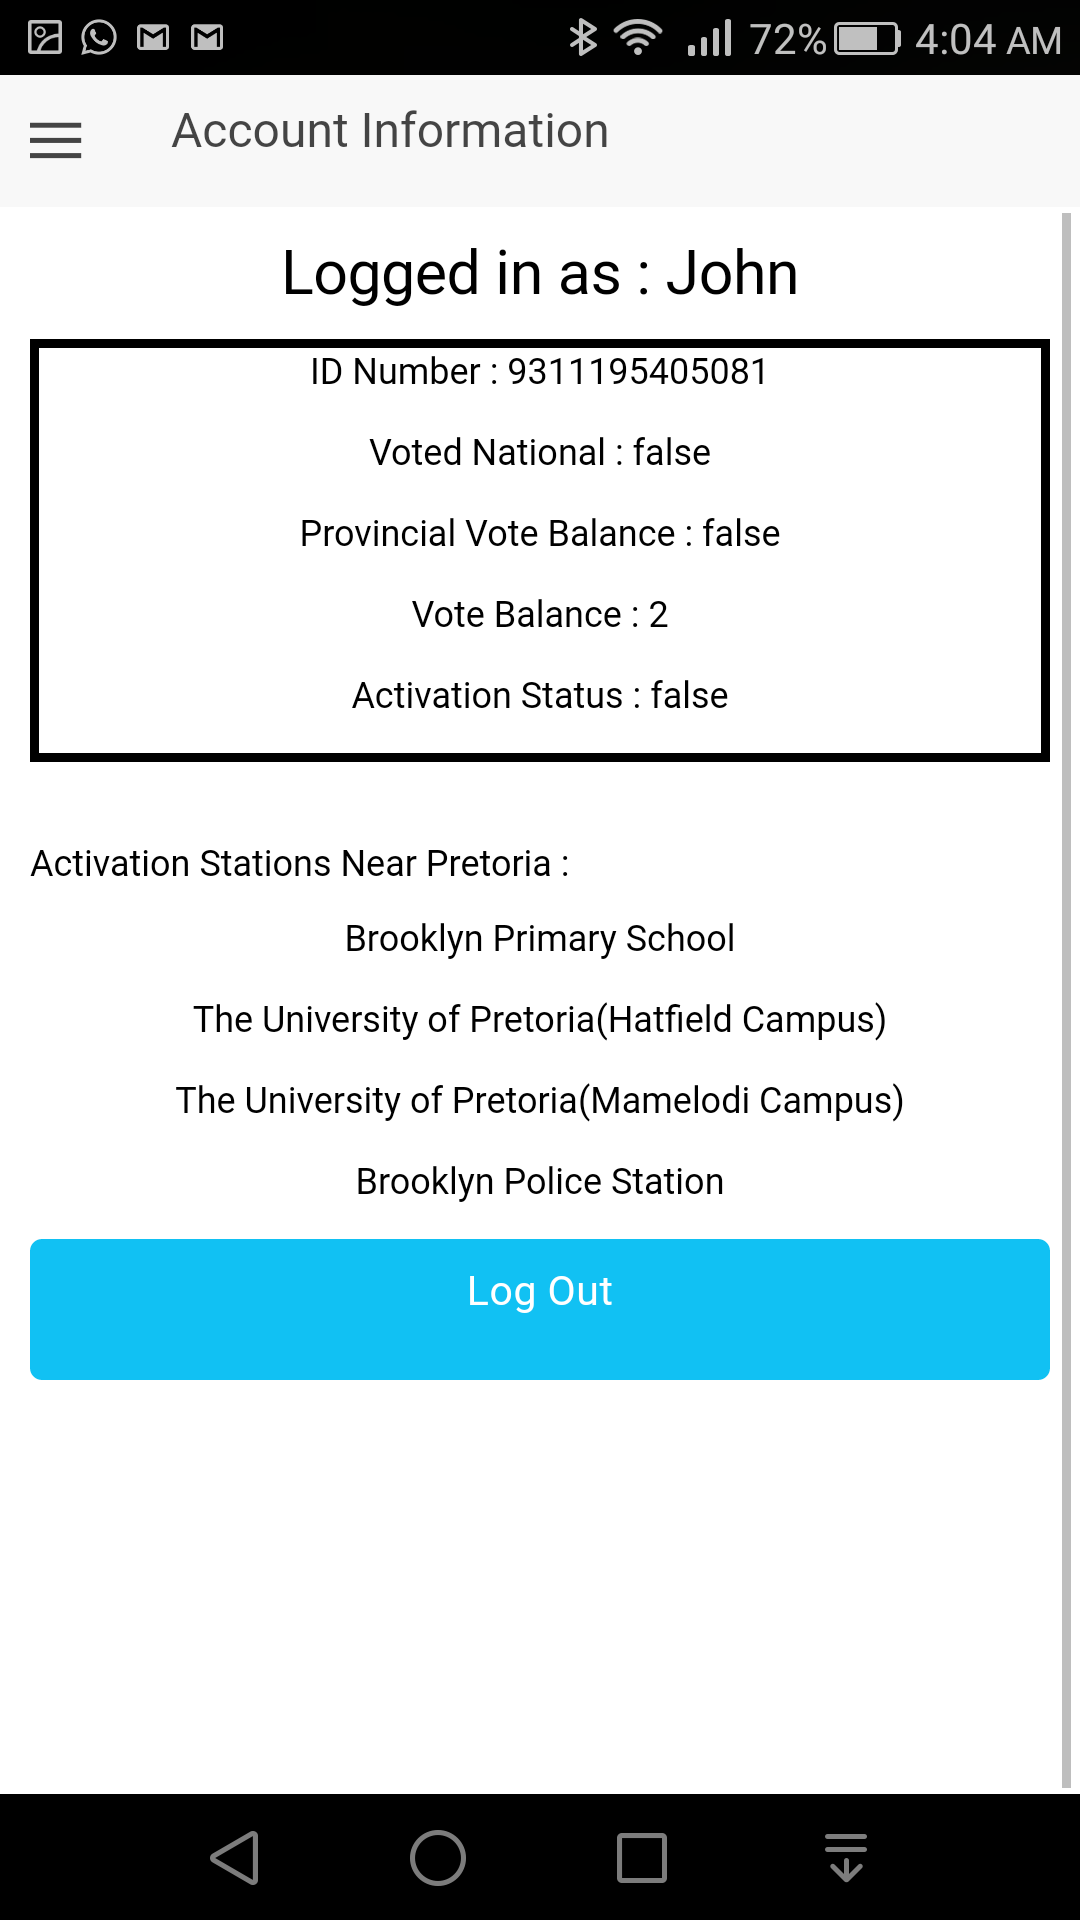
\includegraphics[width=0.3\linewidth]{../Images/UserManual/userinformation.png}
			\caption{Logout Location}
		\end{figure}
	
	\section{Using the System}
	\label{usingthesystem}
	The home screen is the first page after logging into the system.
			\begin{figure}[H]
				\centering
				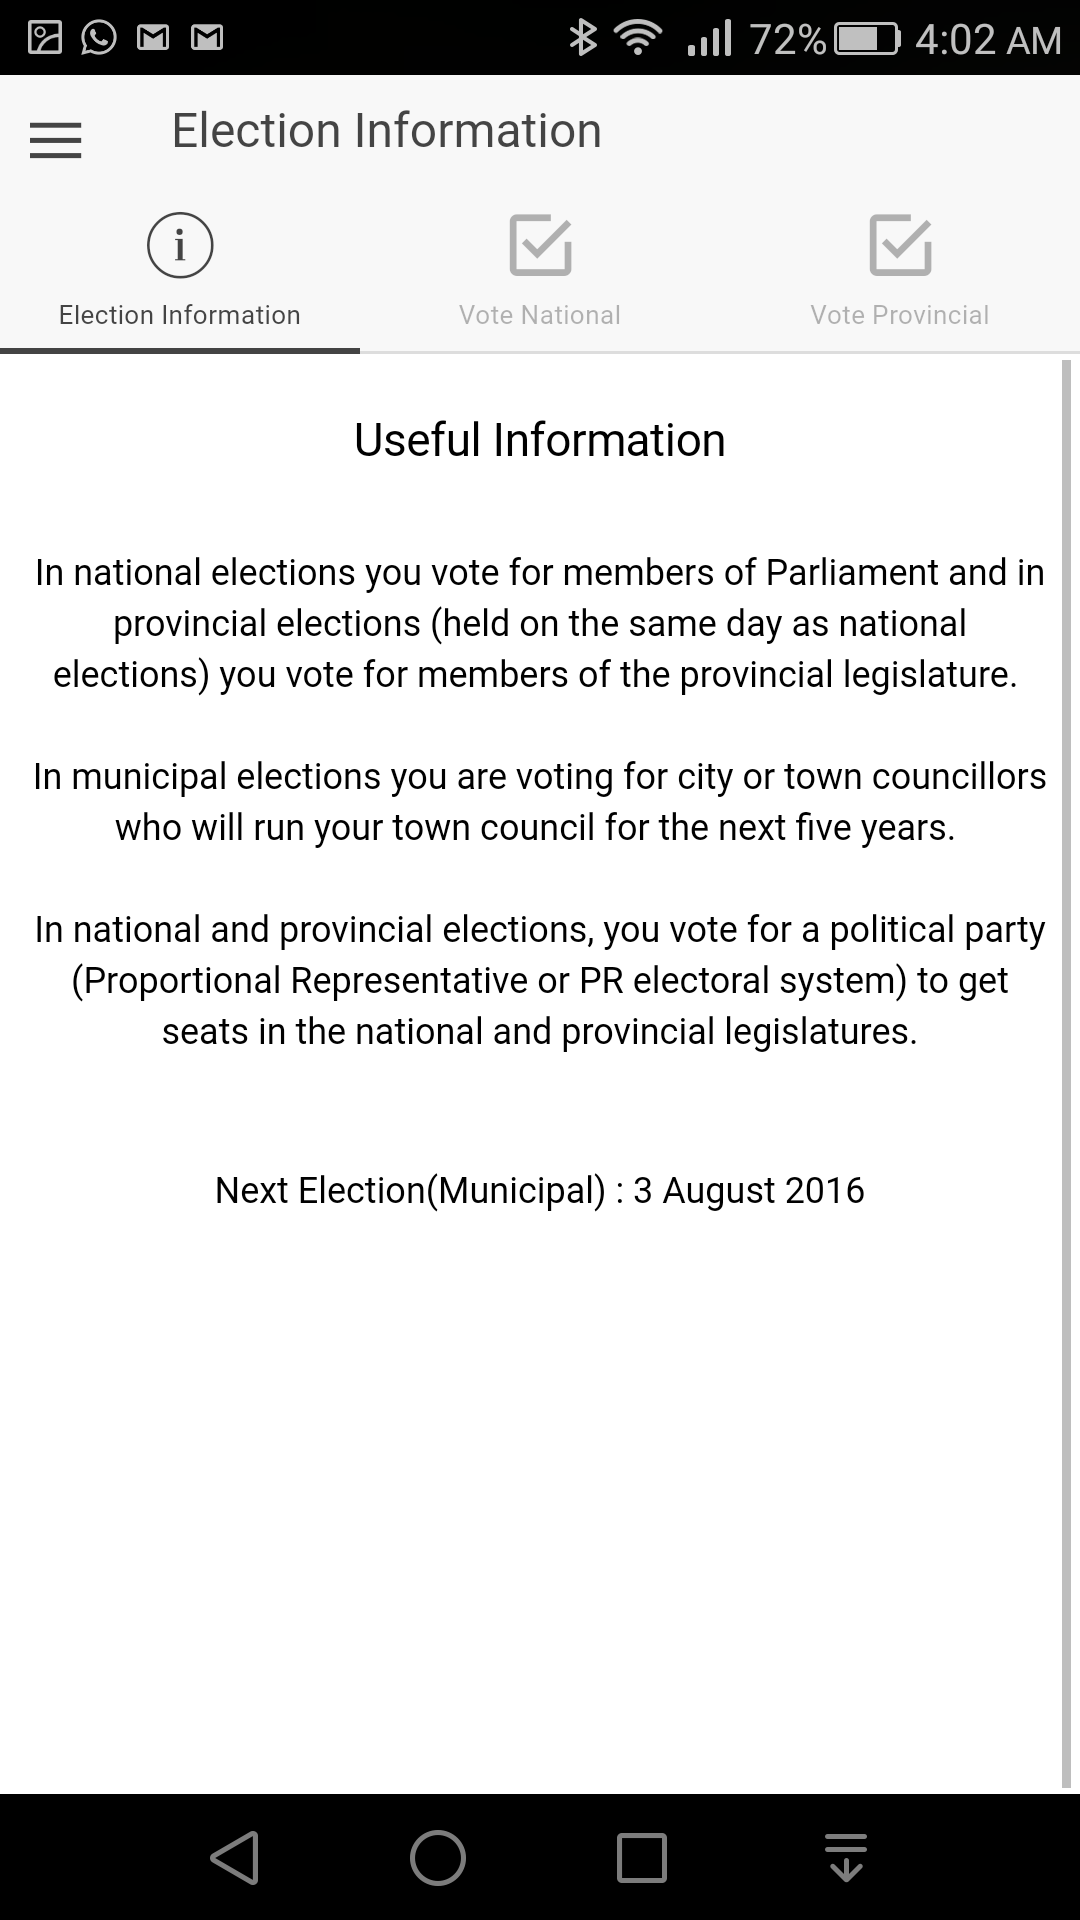
\includegraphics[width=0.3\linewidth]{../Images/UserManual/homescreen.png}
				\caption{Home Screen}
				\label{homescreen}
			\end{figure}
			
			At the top of the screen is a menu with 3 buttons: Election Information, Vote National and Vote Provintial. Each button will redirect the user to another screen. The user is on the Election Information screen directly after logging in. When the user clicks on Vote National, he/she will be taken to a screen of a list of all the running political parties.
			
						\begin{figure}[H]
							\centering
							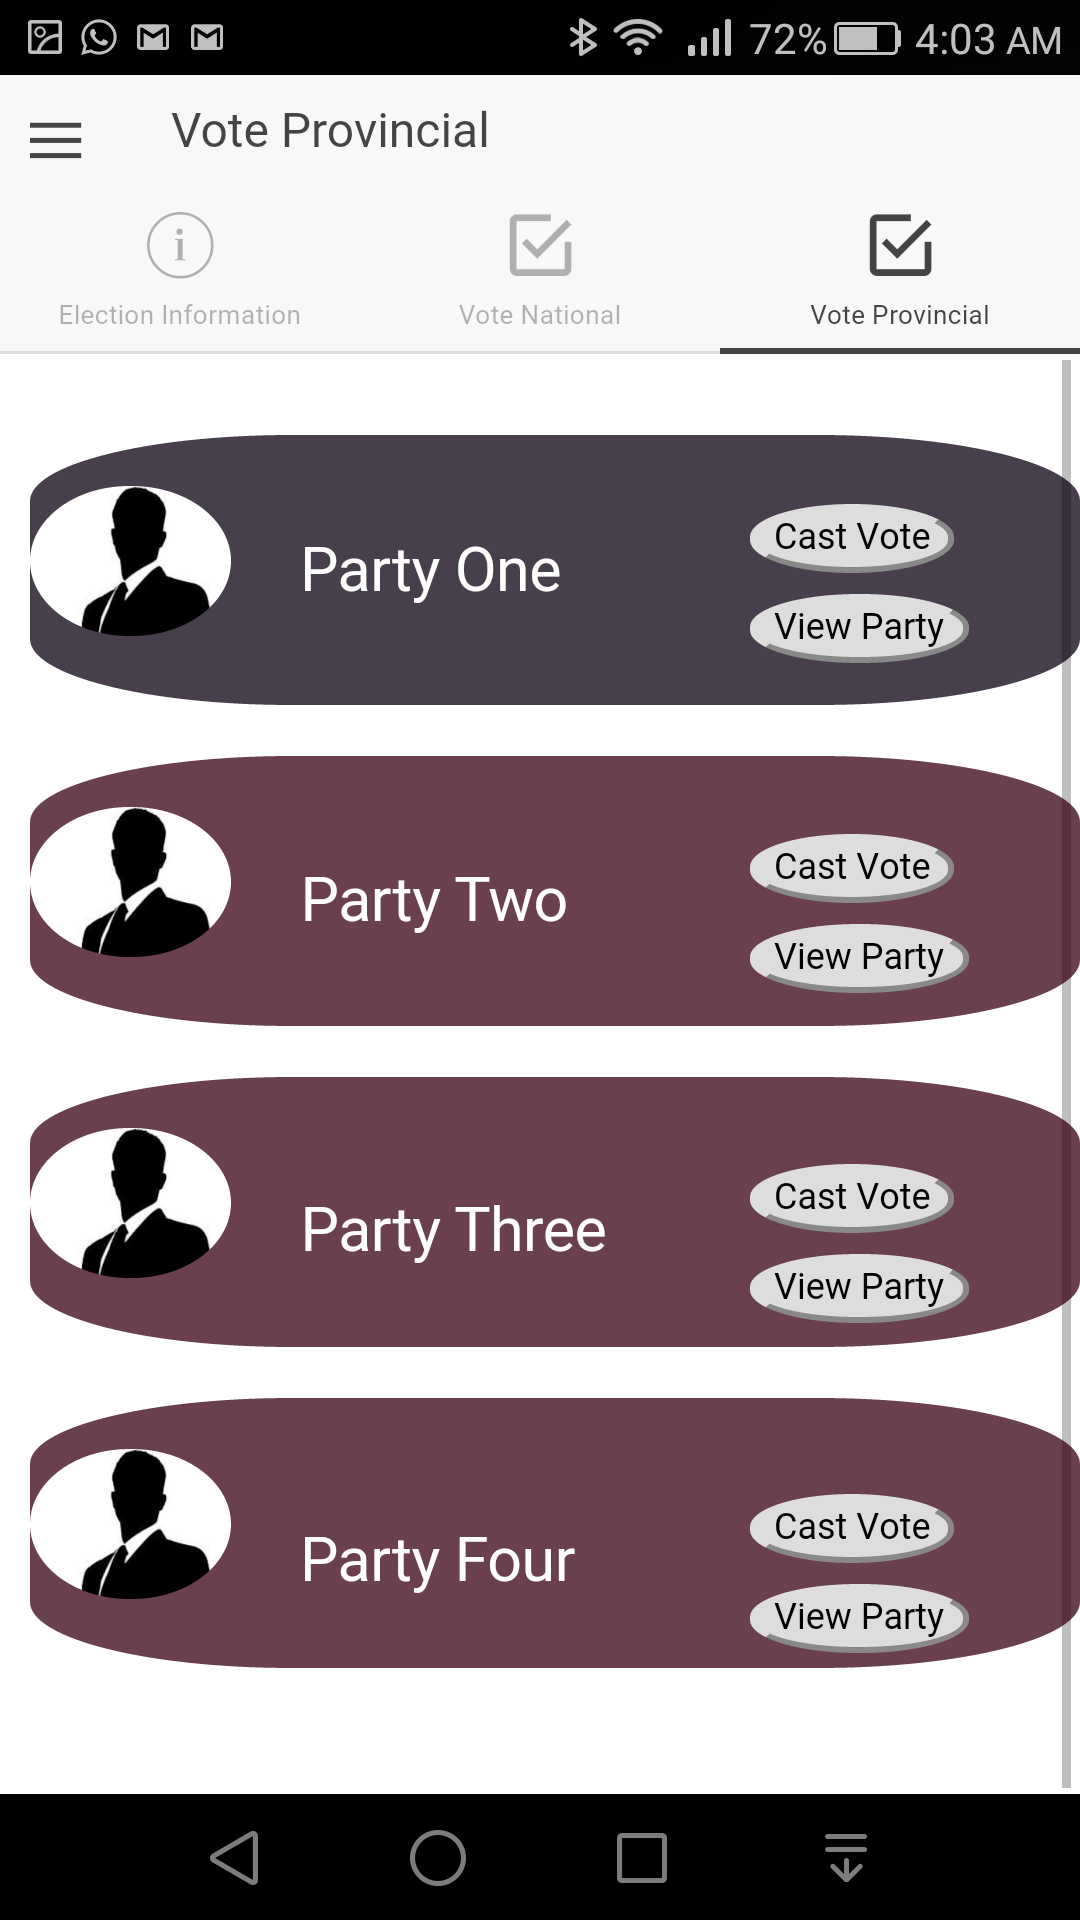
\includegraphics[width=0.3\linewidth]{../Images/UserManual/voteprovintial.png}
							\caption{Vote Provintial}
						\end{figure}
												\begin{figure}[H]
													\centering
													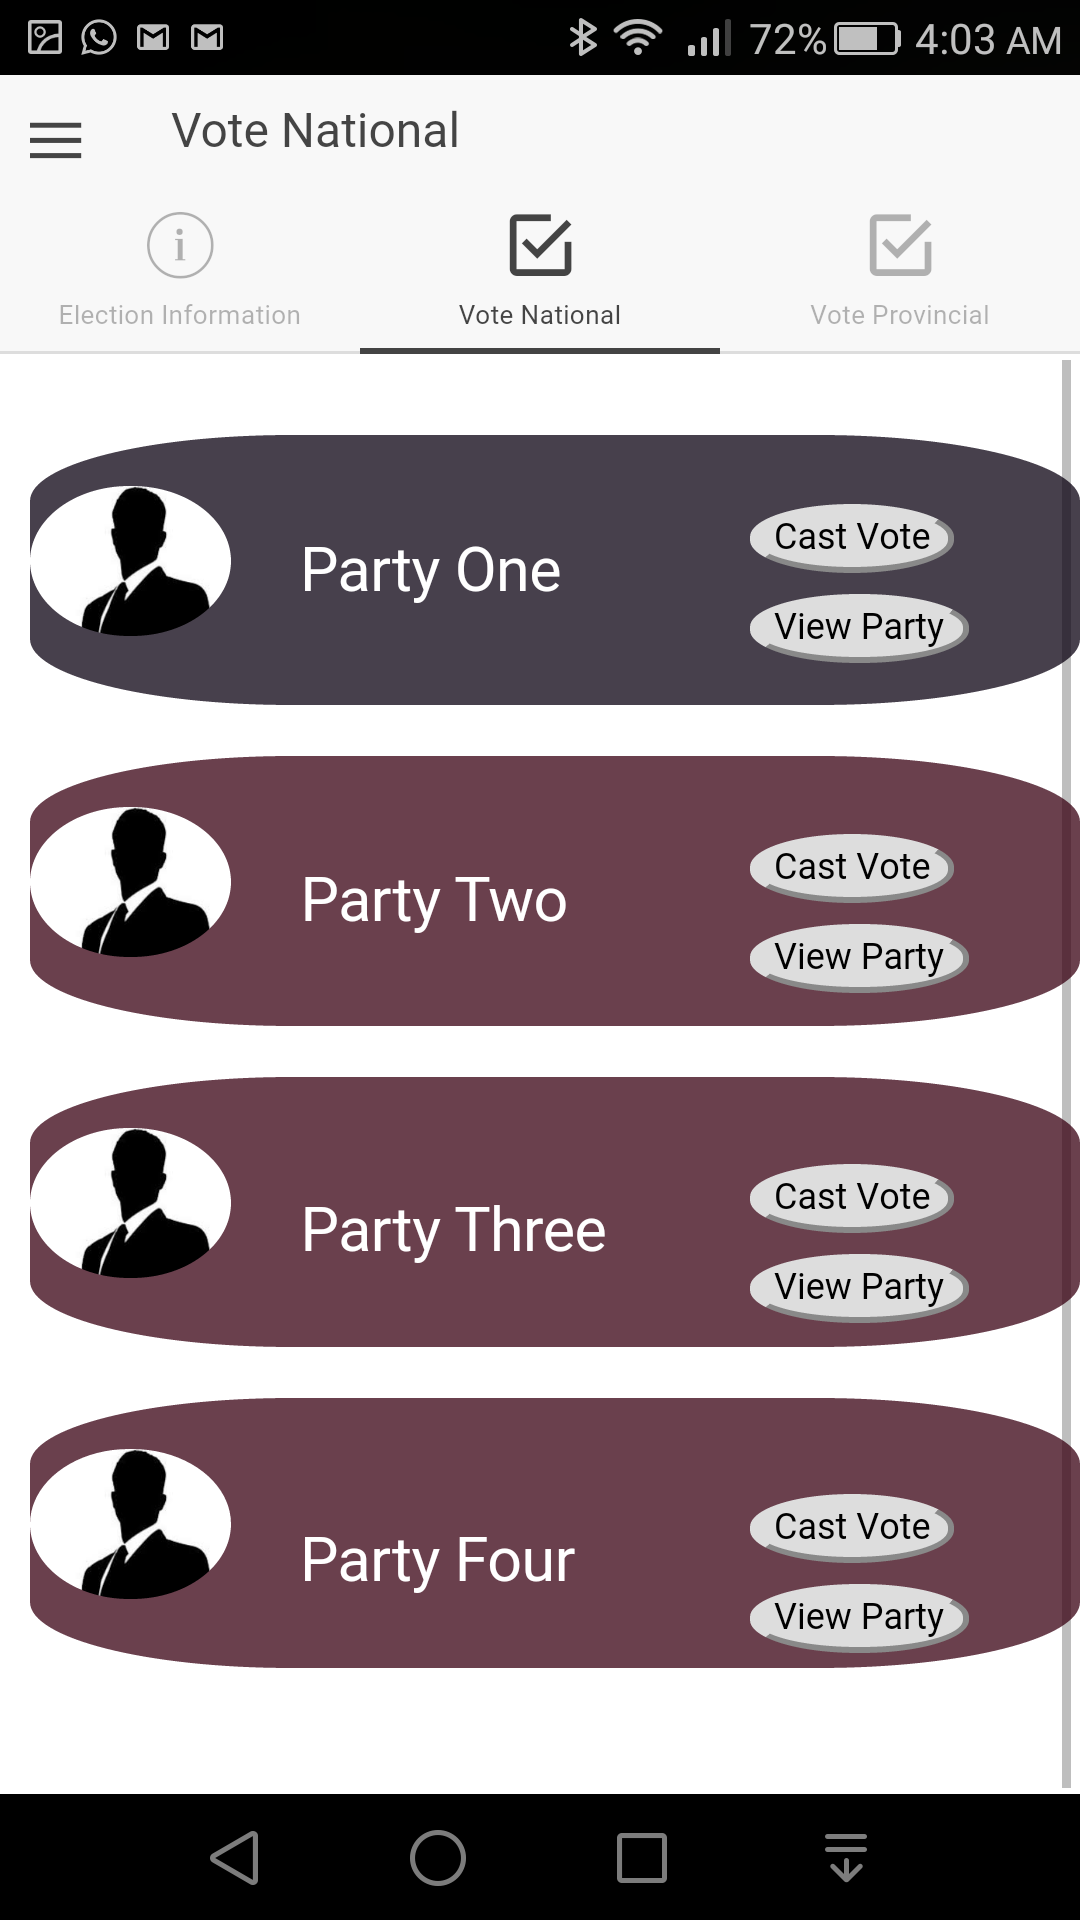
\includegraphics[width=0.3\linewidth]{../Images/UserManual/votenational.png}
													\caption{Vote National}
												\end{figure}
	
		At each of the above screens, the user can view a party's information and cast a vote for a party. The user only has 1 for a national election, and 1 vote for a provintial election.
		\newline\newline
		If a user hasn't voted before, and clicks on "Cast Vote" (either national or provintial) the folowing screen should appear:
		\begin{figure}[H]
			\centering
			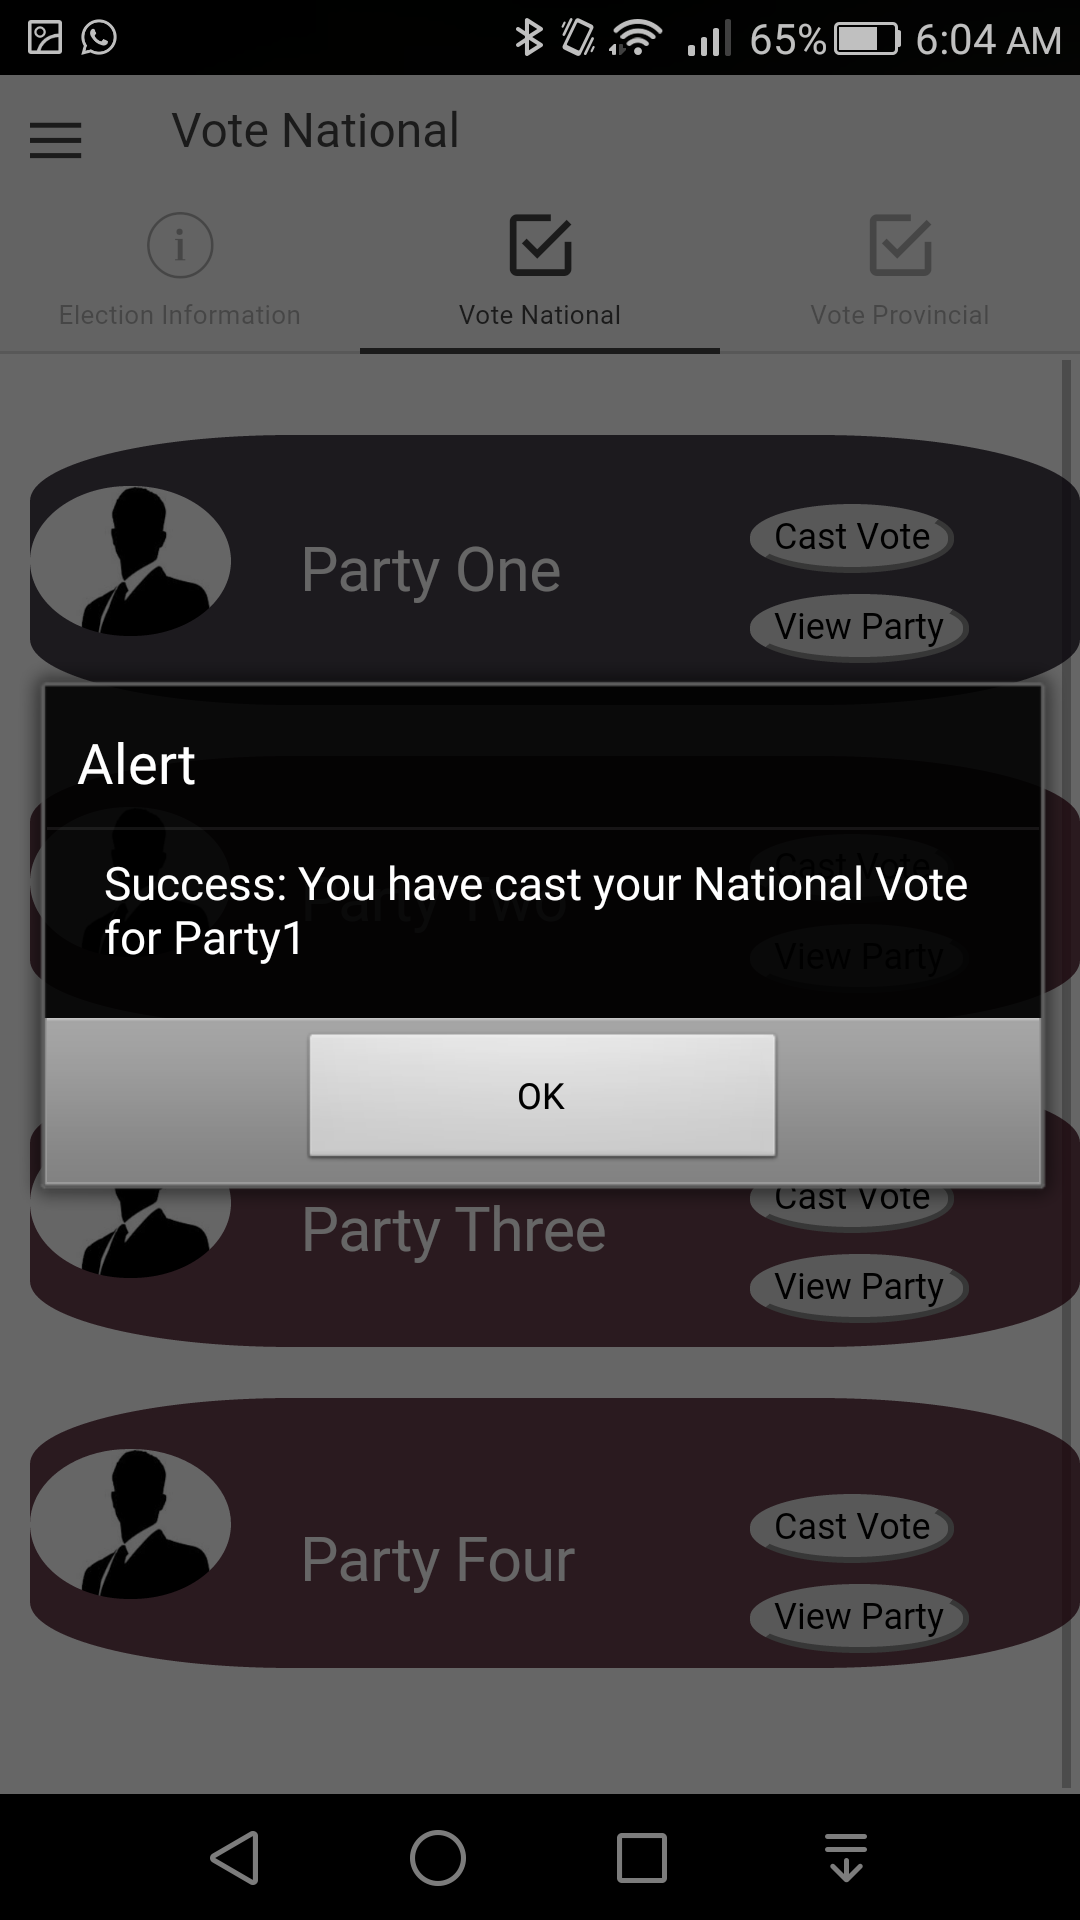
\includegraphics[width=0.3\linewidth]{../Images/UserManual/successvote.png}
			\caption{Successful Vote}
		\end{figure}
		
		The image at figure \ref{alreadyVoted} will be shown if a user has already voted and tries to vote again.
	
		\section{Troubleshooting}
		The backend prevents a user from casting multiple votes. So if a user tries to vote again, the folowing message will appear:
		\begin{figure}[H]
			\centering
			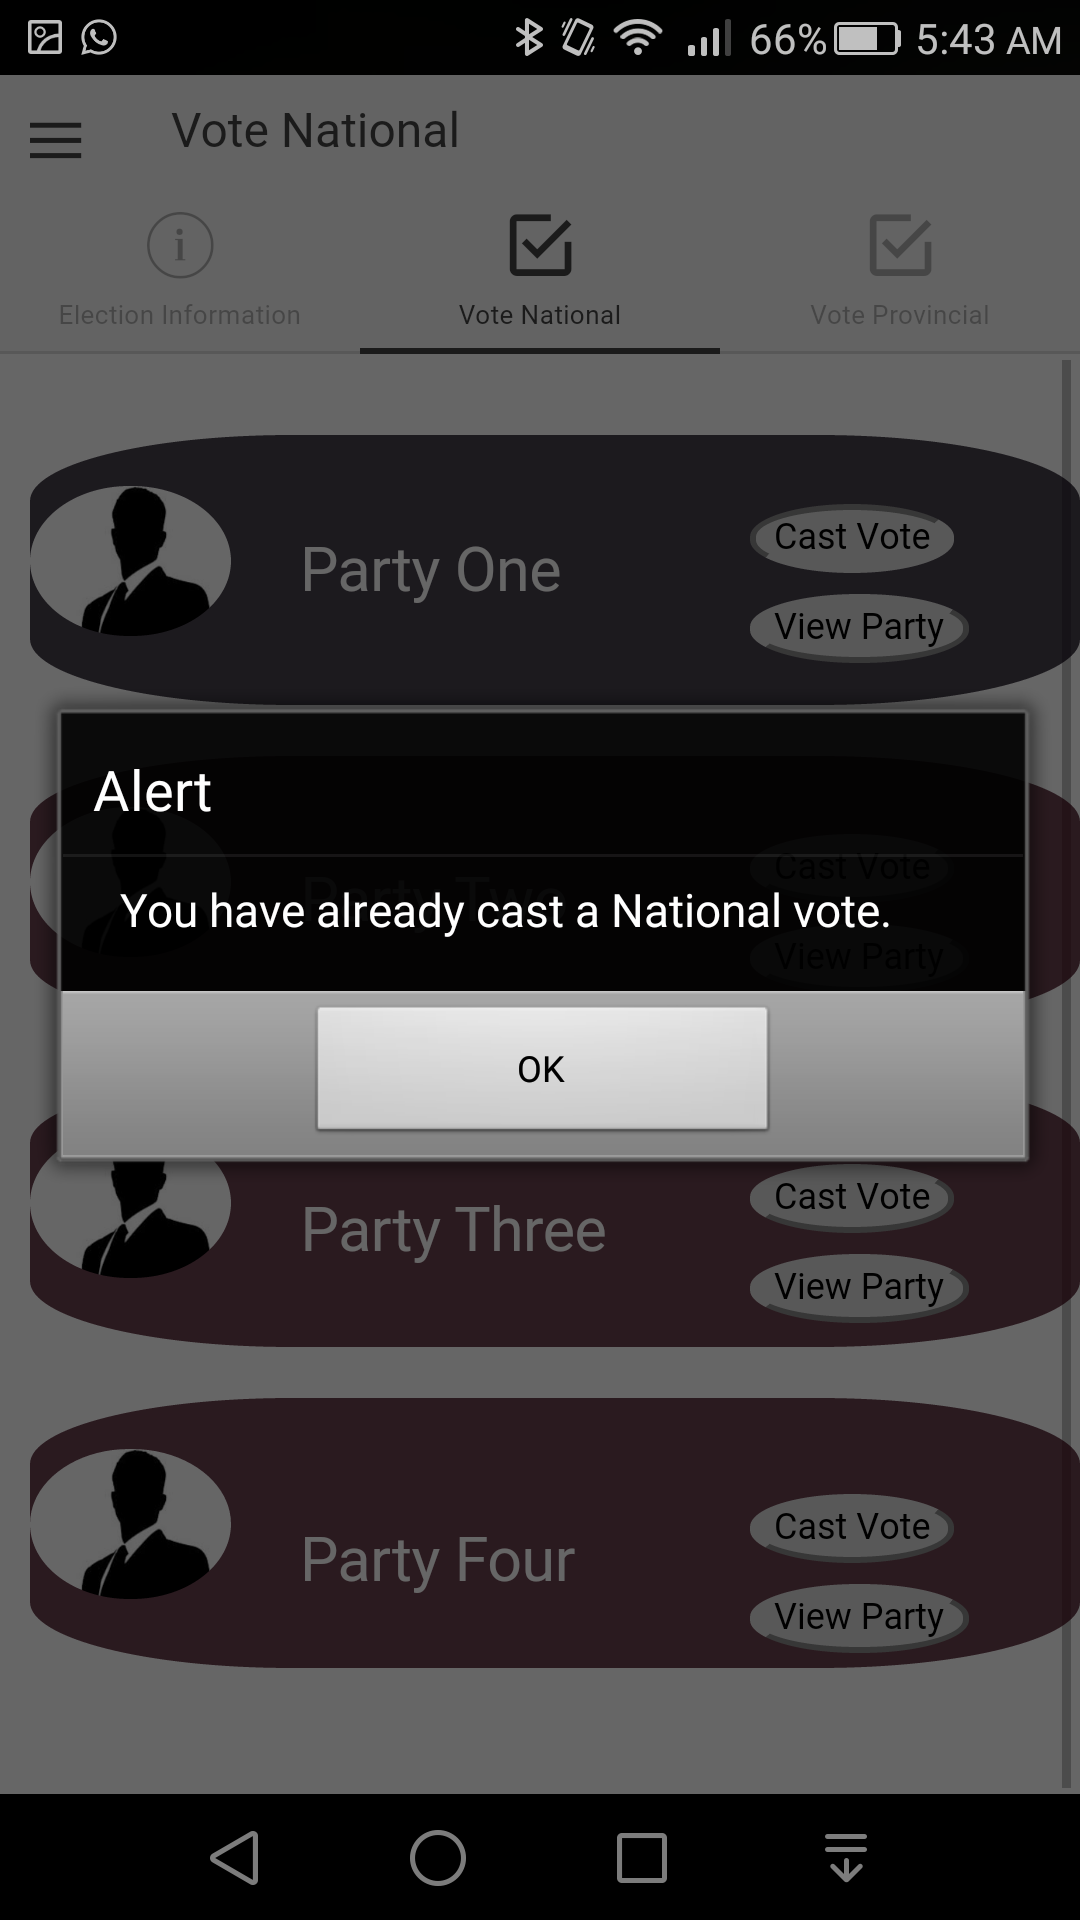
\includegraphics[width=0.3\linewidth]{../Images/UserManual/alreadyvoted.png}
			\caption{Already Voted}
			\label{alreadyVoted}
		\end{figure}
\end{document}